\documentclass[crop,tikz]{standalone}

\tikzset{>=latex}
\usetikzlibrary{calc}
\newcommand{\place}{\vec{r}}
\newcommand{\velocity}{\vec{v}}

\begin{document}
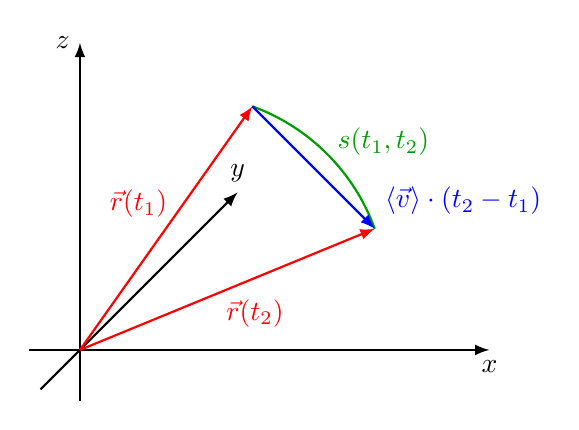
\begin{tikzpicture}[scale=1.3]
  % axes
  \draw[->,thick] (xyz cs:x=-0.5) -- (xyz cs:x=4)  node[below] {$x$};
  \draw[->,thick] (xyz cs:y=-0.5) -- (xyz cs:y=3)  node[left] {$z$};
  \draw[->,thick] (xyz cs:z=1)    -- (xyz cs:z=-4) node[above] {$y$};
  % space point
  \coordinate (r1) at ($(1,0.5)+(70:2)$);
  \coordinate (r2) at ($(1,0.5)+(20:2)$);
  % path
  \draw[thick,black!40!green] (r1) arc (70:20:2);
  \node[right,xshift=0.5em,black!40!green] at ($(1,0.5)+(50:2)$) {$s(t_1,t_2)$};
  % space-point vectors
  \draw[->,thick,red] (xyz cs:x=0) -- node[above,xshift=-1em]{$\place(t_1)$} (r1);
  \draw[->,thick,red] (xyz cs:x=0) -- node[below,xshift=+1em]{$\place(t_2)$} (r2);
  % delta r
  \draw[->,thick,blue] (r1) -- (r2) node[right,yshift=1em]{$\langle\velocity\rangle\cdot(t_2-t_1)$};
\end{tikzpicture}
\end{document}
